%% Begin slides template file
\documentclass[11pt,t,usepdftitle=false,aspectratio=169]{beamer}
%% ------------------------------------------------------------------
%% - aspectratio=43: Set paper aspect ratio to 4:3.
%% - aspectratio=169: Set paper aspect ratio to 16:9.
%% ------------------------------------------------------------------

\usetheme[nototalframenumber,foot,logo]{uibk}

\title[Segfault Slayer]{Progress Update 2: Segfault Slayer}

\author[Schmölz Lukas, Schöpf Emanuel, Schweigl Dominik]{Schmölz Lukas, Schöpf Emanuel, \textbf{Schweigl Dominik}}

\headerimage{3}

\begin{document}

\section{Bookmark Title}
\subsection{Overview}

\begin{frame}
	\frametitle{Game Overview}

	\textbf{Game Idea:}
	\begin{itemize}
		\item Metroidvania-style 2D side-scroller
		\item Player fights programming concepts and bugs (mainly C++ related)
		\item Playful, Pixel-theme (e.g. ASCII-Art for textures)
	\end{itemize}

	\bigskip

	\textbf{World Design:}
	\begin{itemize}
		\item First Area: Hardware with Logic Operators
		\item Second Area: Programming with loops and other concepts
	\end{itemize}
\end{frame}

\begin{frame}{Previous Goals}
	\vspace{1em}
	\begin{itemize}
		\item Proper rendering
		\item Proper physics
		\item Additional content (player, enemies, health, rooms, \ldots)
	\end{itemize}
\end{frame}

\begin{frame}{Textures \& Rooms}
	\begin{columns}[T]
		\begin{column}{0.55\textwidth}
			\small
			\textbf{Improved Tile Textures}
			\begin{itemize}
				\item Pixel art tiles --- ongoing, more tiles being added
				\item Pixellab explored for tile creation
			\end{itemize}

			\vspace{1em}

			\textbf{Multiple Rooms}
			\begin{itemize}
				\item World split into separate room files
				\item Room switching via coordinate check
				\item To be replaced with teleport tiles
			\end{itemize}
		\end{column}

		\begin{column}{0.4\textwidth}
			\vspace{-1em}
			\begin{center}
				
\includegraphics[width=0.33\linewidth]{_images/top1.png}
				
\includegraphics[width=0.33\linewidth]{_images/top2.png}\\[4pt]
				
\includegraphics[width=0.33\linewidth]{_images/left_edge.png}
				
\includegraphics[width=0.33\linewidth]{_images/right_edge.png}\\[4pt]
				
\includegraphics[width=0.33\linewidth]{_images/structure.png}
			\end{center}
		\end{column}
	\end{columns}
\end{frame}

\begin{frame}{Asset Manager}
	\begin{columns}[T]
		\begin{column}{0.55\textwidth}
			\small
			\textbf{Centralised Texture Loading}
			\begin{itemize}
				\item Singleton \texttt{AssetManager} owns all textures
				\item \texttt{TextureAsset} enum as type-safe asset keys
				\item No \texttt{loadFromFile} calls in entity code
				\item Textures loaded once, shared by \texttt{const} reference
			\end{itemize}
		\end{column}

		\begin{column}{0.4\textwidth}
			\small
			\vspace{2em}
			\texttt{AssetManager::getInstance()} \\
			\texttt{\ \ .getTexture(PLAYER\_HEAD);}
		\end{column}
	\end{columns}
\end{frame}

\begin{frame}{Player --- Sprite System}
	\begin{columns}[T]
		\begin{column}{0.45\textwidth}
			\small
			\textbf{Three-Layer Sprite Architecture}
			\begin{itemize}
				\item \textbf{Lower body} --- motion animations
				\item \textbf{Upper body} --- motion animations / attack animations
				\item \textbf{Head} --- hat / no-hat (managed by Player)
			\end{itemize}

			\vspace{1em}

			\textbf{Per-Frame Offset System}
			\begin{itemize}
				\item Each state exposes \texttt{getHeadOffset()} and \texttt{getUpperBodyOffset()} per frame
				\item Enables composition across all states
			\end{itemize}
		\end{column}

		\begin{column}{0.5\textwidth}
			\vspace{-1em}
			\begin{columns}[T]
				\begin{column}{0.3\linewidth}
					\centering
					
\includegraphics[width=\linewidth]{_images/idle_lower_body_extended.png}\\[3pt]
					
\includegraphics[width=\linewidth]{_images/run_lower_body_extended.png}\\[3pt]
					
\includegraphics[width=\linewidth]{_images/walk_lower_body_extended.png}
				\end{column}
				\begin{column}{0.3\linewidth}
					\centering
					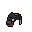
\includegraphics[width=\linewidth]{_images/idle_upper_body_extended_no_head.png}\\[3pt]
					
\includegraphics[width=\linewidth]{_images/run_upper_body_extended_no_head.png}\\[3pt]
					
\includegraphics[width=\linewidth]{_images/attack_swing_upper_body_extended_no_head.png}
				\end{column}
				\begin{column}{0.3\linewidth}
					\centering
					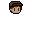
\includegraphics[width=\linewidth]{_images/head_hat.png}\\[3pt]
					
\includegraphics[width=\linewidth]{_images/head.png}\\[3pt]
					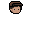
\includegraphics[width=\linewidth]{_images/head_blink.png}
				\end{column}
			\end{columns}
		\end{column}
	\end{columns}
\end{frame}

\begin{frame}{Player --- Hat Throw Ability}
	\begin{columns}[T]
		\begin{column}{0.45\textwidth}
			\small
			\textbf{New Player Ability}
			\begin{itemize}
				\item Player throws hat as a projectile
				\item Head switches to hatless sprite once hat is taken off, checked via \texttt{isHatOnHead()}
				\item Separate \texttt{HatProjectile} entity
				\item Throw speed and distance adjusted based on player speed
			\end{itemize}
		\end{column}

		\begin{column}{0.55\textwidth}
			\begin{flushright}
				\vspace{-1em}
				
\includegraphics[width=\linewidth]{../../assets/images/player/attack_throw_hat.png}

				\vspace{2em}
				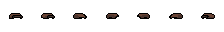
\includegraphics[width=\linewidth]{../../assets/images/player/hat_projectile.png}
			\end{flushright}
		\end{column}
	\end{columns}
\end{frame}

\begin{frame}{Menu System}
	\begin{columns}[T]
		\begin{column}{0.5\textwidth}
			\small
			\textbf{Stack-Based Scene Architecture}
			\begin{itemize}
				\item \texttt{Scene} interface pushed/popped on a stack
				\item Game logic moved to \texttt{GameScene}
				\item \texttt{MenuScene} base class for menus
				\item \textbf{Main Menu} with background image
				\item \textbf{Pause Menu} pushed on top of \texttt{GameScene}
			\end{itemize}
		\end{column}

		\begin{column}{0.45\textwidth}
			\begin{flushright}
				\vspace{-2em}
				
\includegraphics[width=\linewidth]{./_images/main_menu_background.png}
				\vspace{1em}
				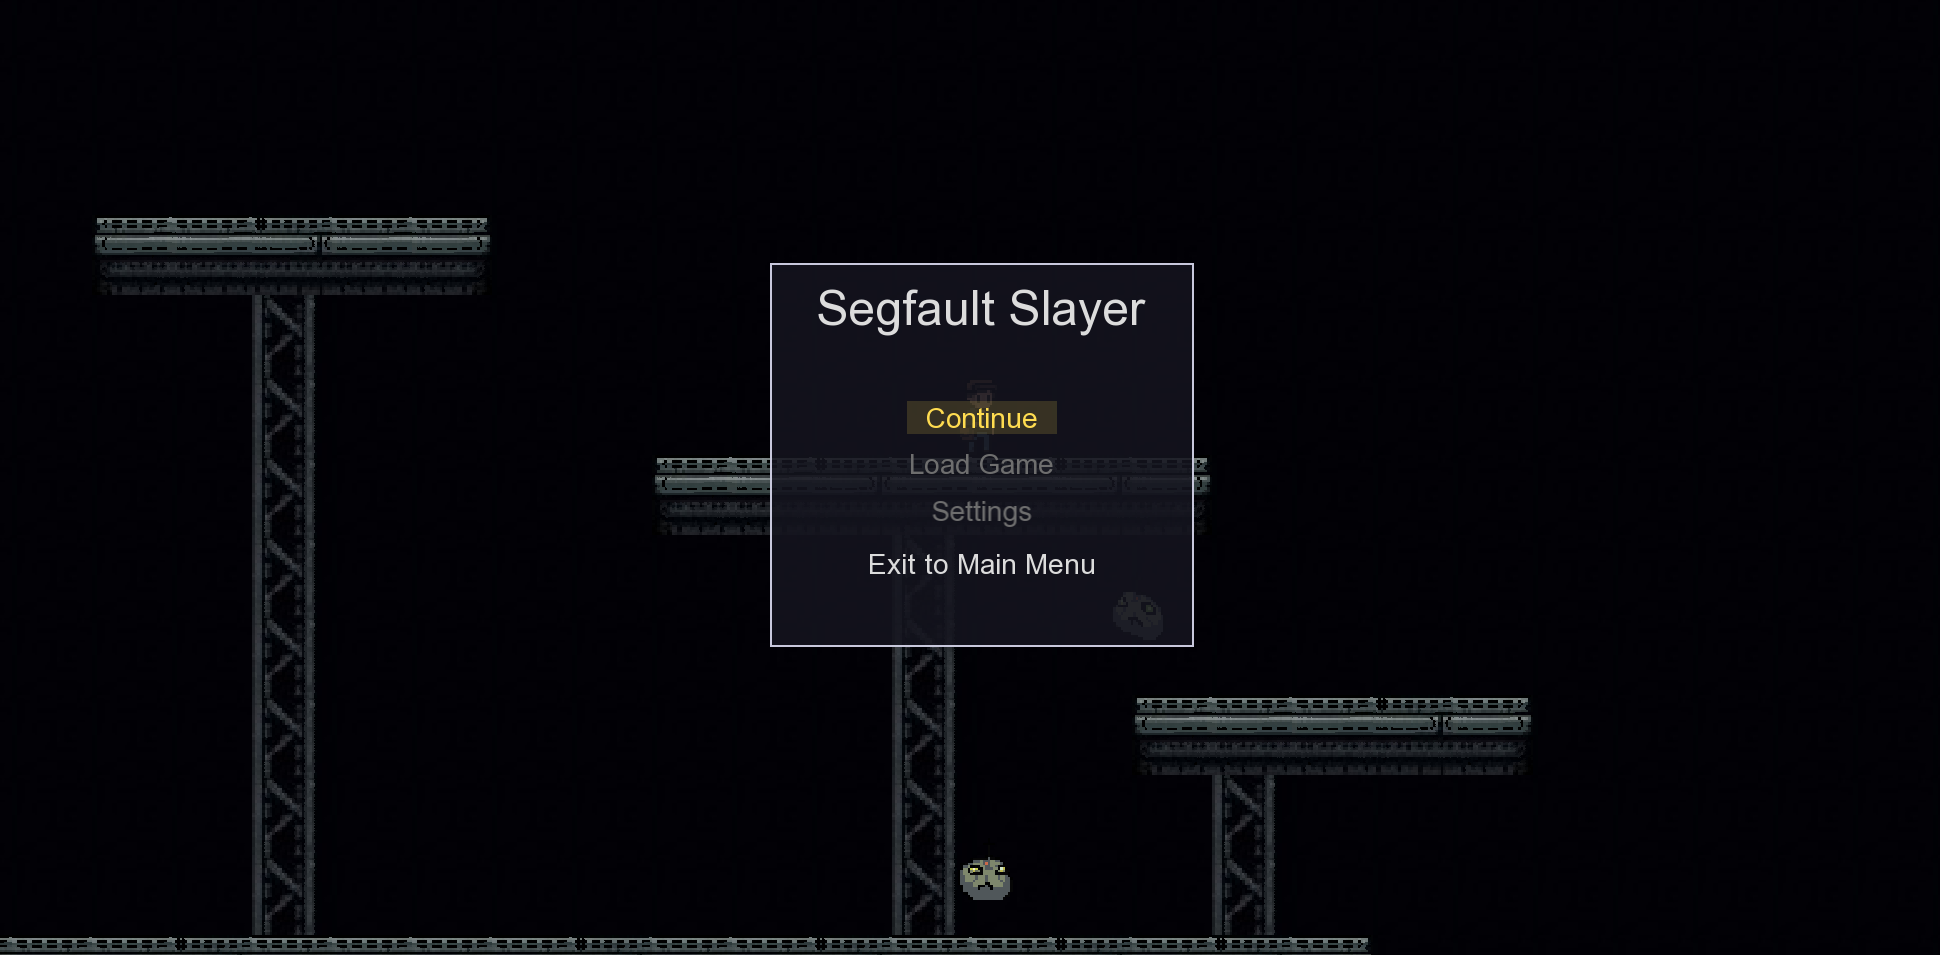
\includegraphics[width=\linewidth]{_images/pause_menu.png}
			\end{flushright}
		\end{column}
	\end{columns}
\end{frame}

\begin{frame}[plain,c]
	\begin{center}
		\Huge{Demo \& Code Review}
	\end{center}
\end{frame}

\begin{frame}{Next Steps}
	\vspace{1em}
	\begin{itemize}
		\item Player/Enemy Health System
		\item More Enemies / Boss
		\item Keyboard Binding Management
		\item Entitiespawns in the Map
		\item Game Saves
	\end{itemize}
\end{frame}

\end{document}
